\documentclass[../../main.tex]{subfiles}
\captionsetup[table]{name=Tabla}
\begin{document}
\begin{frame}{Planificación de la producción}{}
  Una empresa produce filtros para monitores de ordenador formados por tres capas, una intermedia de calidad $A$ y otras dos exteriores de calidad $B$ que envuelven a la anterior. Ambas calidades se consiguen con diferentes mezclas de fibra de vidrio y resina de las que el fabricante dispone  por semana de 700 y 900 toneladas ($t$), respectivamente. La empresa posee cuatro plantas de producción que utilizan procedimientos de fabricación que difieren en las cantidades de materia prima que utilizan. Las cantidades necesarias de materia prima por operación para cada planta que se pueden llevar a cabo total o parcialmente así como el número de capas producidas de uno y otro tipo, se tienen en la Tabla~\ref{tab:info}.

\end{frame}

\begin{frame}{Planificación de la producción}{}

  \begin{table}
    \caption[requerimientos]{\label{tab:info}Requerimientos para la fabricación de filtros para PC.}
    \centering
    \begin{tabular}{ccccc}
      \toprule
      ~ & \multicolumn{2}{c}{$t$ requeridas} & \multicolumn{2}{c}{Capas producidas}\\
      ~& \multicolumn{2}{c}{por operación}& \multicolumn{2}{c}{por operación}\\
      \cmidrule{2-5}
      Planta& Vidrio& Resina& Tipo $A$& Tipo $B$\\
      \midrule
      1& 15& 19& 2& 5\\
      2& 14& 20& 3& 7\\
      3& 16& 15& 5& 4\\
      4 & 12& 18& 4& 4\\
      \bottomrule
    \end{tabular}

  \end{table}
  Formular un modelo de programación lineal para determinar el número de operaciones a realizar en cada planta de manera que sea máximo el número total de filtros fabricados
\end{frame}

\begin{frame}{Planificación de la producción}{}
  Para la formulación de la función objetivo hay que tomar en cuenta que para formar un filtro se necesita 1 unidad de $A$ y dos unidades de $B$, así, por ejemplo, si decidimos ejecutar una operación en cada planta obtendríamos 14 unidades de $A$ y 20 unidades de $B$ y con estas unidades solo se pueden elaborar 10 filtros.

  {\centering
    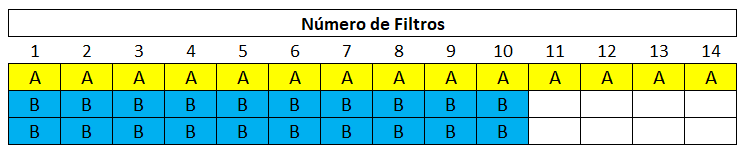
\includegraphics[scale=0.35]{05_production-planning.png}
    \par}

  \begin{columns}
    \column{0.4\textwidth}
      \begin{align*}
    A = 2(1) + 3(1) + 5(1) + 4(1)  &= 14\\
    B = 5(1) + 7(1) + 4(1) + 4(1)  &= 20\\
  \end{align*}
  \column{0.5\textwidth}
      \begin{align*}
        Z_A &= \nicefrac{A}{1} = \nicefrac{14}{1} = 14\\
        Z_B &= \nicefrac{B}{2} = \nicefrac{20}{2} = 10\\[3mm]
        Z &= \min\{Z_A, Z_B \}\\
        &= \min\{14, 10 \} = 10
      \end{align*}
  \end{columns}



  
\end{frame}

\end{document}